\documentclass[11pt]{article}

\usepackage[margin=1in]{geometry}
\usepackage[T1]{fontenc}
\usepackage[utf8]{inputenc}
\usepackage{amsmath,amssymb,amsthm}
\usepackage{booktabs}
\usepackage{graphicx}
\usepackage{natbib}
\usepackage{hyperref}
\usepackage{xcolor}

\graphicspath{{figures/}{../outputs/real_well_f03/direct_ub/runs/f03_full_gr_only_clp_csgm_ridge/figures/}}

\newtheorem{assumption}{Assumption}
\newtheorem{proposition}{Proposition}
\newtheorem{corollary}{Corollary}
\theoremstyle{remark}
\newtheorem{remark}{Remark}

\title{Conditional Latent-Prior Generative Compressed Sensing for Petrophysical Property Estimation from Sparse Core Measurements}
\author{Author names omitted for review}
\date{}

\begin{document}

\maketitle

\begin{abstract}
Dense well logs provide continuous indirect observations of subsurface
properties, whereas core measurements are sparse, expensive, and usually
available only at selected depths. Direct supervised models can exploit log
features, but they often use sparse target-well measurements only as additional
inputs. Classical compressed sensing provides a principled measurement
consistency mechanism, but its fixed-basis sparsity assumption can be too rigid
for cross-well petrophysical prediction. We propose Conditional Latent-Prior
Compressed Sensing with Generative Models (CLP-CSGM), a method that learns a
generative manifold of target-property windows and uses well logs to predict a
latent prior. Sparse core measurements then refine the reconstruction through a
test-time latent inverse problem. In low-data cross-well clay-volume prediction,
CLP-CSGM Ridge improves over a direct autoencoder baseline in all tested
training-size and measurement-ratio cells, reducing mean RMSE from 0.01905 to
0.01397. In a real-well F03-4 porosity benchmark using only gamma ray as dense
input, CLP-CSGM Ridge attains the best average RMSE, with strongest gains in
the sparsest measurement regimes.
\end{abstract}

\section{Introduction}
\label{sec:introduction}

Petrophysical property estimation is a central task in reservoir
characterization. Wireline logs are dense along depth and can be acquired in
most wells, but properties such as porosity, clay volume, or shale volume are
usually calibrated by core or laboratory measurements that are sparse and
expensive \citep{ellis2007well,asquith2004basic}. This mismatch creates a
recurring inverse problem: a model must infer a continuous target-property
profile from dense indirect logs while honoring a small number of direct
measurements in the target well.

Machine-learning regressors are attractive in this setting because they can
learn nonlinear relations between logs and target properties from previously
interpreted wells \citep{bishop2006pattern}. However, a direct map from logs to
targets may underuse sparse core observations available in the target well. A
common direct workaround is to concatenate the sparse measurement vector with
the logs and train a supervised model from \([u,b]\) to \(y\). Although this can
be competitive, it treats the sparse measurements as features rather than as
measurement evidence about the reconstructed signal.

Compressed sensing (CS) offers the complementary perspective: measurements
should constrain the reconstruction through a forward model
\citep{donoho2006compressed,candes2006robust,candes2006stable}. Classical CS
usually assumes sparsity in a fixed basis, such as wavelets or discrete cosine
atoms. In cross-well petrophysical prediction, this assumption can be too
restrictive. Geological variability is not necessarily sparse in a universal
basis, and fixed-basis residual correction may fail to outperform strong
supervised baselines.

Compressed sensing with generative models (CSGM) replaces fixed-basis sparsity
with a learned generative range \citep{bora2017compressed}. Instead of seeking
a sparse coefficient vector, one searches for a latent code \(z\) such that the
generated signal \(G(z)\) matches the measurements. This is well aligned with
petrophysical windows: the decoder can represent plausible target profiles,
while sparse core observations can select the profile that is consistent with
the target-well evidence.

This paper proposes Conditional Latent-Prior CSGM (CLP-CSGM) for
petrophysical property estimation from dense logs and sparse core measurements.
The method trains an autoencoder decoder \(G\) on target-property windows and a
ridge prior \(h\) that maps the dense log window \(u\) to an initial latent
code \(z_0=h(u)\). At test time, the final latent code is obtained by solving a
measurement-consistent inverse problem,
\begin{equation}
  \hat z =
  \arg\min_z
  \|M G(z)-b\|_2^2
  + \lambda \|z-z_0(u)\|_2^2,
  \qquad
  \hat y = G(\hat z).
  \label{eq:intro_clp_csgm}
\end{equation}
The first term penalizes sparse core inconsistency; the second term keeps the
solution close to the log-conditioned latent prior.

The contributions are:
\begin{itemize}
  \item We formulate CLP-CSGM, a conditional generative compressed sensing
  method for petrophysical property windows.
  \item We provide a theoretical interpretation of the objective as a
  Tikhonov/MAP latent inverse problem and relate it to standard CSGM guarantees.
  \item We evaluate the method in low-data cross-well clay-volume prediction
  and in a real-well F03-4 GR-only porosity stress test.
  \item We show that CLP-CSGM Ridge improves over strong direct baselines in
  sparse-measurement regimes, and we use structural ablations to show that both
  the conditional latent prior and the sparse-measurement term are needed.
\end{itemize}

The remainder of the paper reviews related work, defines CLP-CSGM, describes the
datasets and experimental protocol, reports quantitative and ablation results,
and discusses the regimes in which the method is most appropriate.

\section{Related work}
\label{sec:related_work}

\paragraph{Petrophysical prediction from logs.}
Well logs provide indirect but dense measurements of rock and fluid properties,
and core-calibrated interpretation is a standard component of petrophysical
analysis \citep{ellis2007well,asquith2004basic}. Data-driven models are now
widely used to map logs to porosity, permeability, saturation, or shale-related
properties \citep{ahmadi2019comparison,wood2020predicting}. These models are
effective when the training distribution is representative and labels are
sufficient, but their usual prediction form is purely supervised. Sparse
measurements in the target well are commonly used as additional features or for
post-hoc calibration, not as explicit constraints in a forward measurement
model.

\paragraph{Sparse compressed sensing.}
Classical compressed sensing reconstructs signals from incomplete linear
measurements by assuming sparsity or compressibility in a known representation
\citep{donoho2006compressed,candes2006robust,candes2006stable}. This view is
appealing for sparse core assimilation because the measurement operator is
known: a row of \(M\) selects the depths where the target was observed. Its
limitation is the structural prior. A fixed basis can be too restrictive for
cross-well petrophysical windows, where changes in depositional setting,
diagenesis, and log-response calibration may create variability that is not
sparse in a universal transform.

\paragraph{Generative priors for inverse problems.}
CSGM replaces the sparse basis with the range of a trained generator
\citep{bora2017compressed}. The unknown signal is represented as \(G(z)\), and
reconstruction searches over \(z\) to minimize measurement mismatch.
\citet{bora2017compressed} established recovery guarantees under set-restricted
eigenvalue conditions and showed that generative priors can require fewer
measurements than sparsity priors in image experiments. Subsequent work studied
the power and limitations of generative compressed sensing
\citep{kamath2020power}, invertible generative priors for inverse problems
\citep{asim2020invertible}, and untrained architectural priors
\citep{ulyanov2018deep}. These works support the central idea that an inverse
problem can be solved by searching a structured generative representation rather
than a fixed sparse basis.

% \paragraph{Conditional generative priors and learned inverse problems.}
% Conditional generative models use auxiliary information to guide generation,
% for example through conditional adversarial models \citep{mirza2014conditional}
% or conditional variational models \citep{sohn2015learning}. In parallel, learned
% inverse-problem methods use neural models as reconstruction maps, regularizers,
% or priors \citep{ongie2020deep,lucas2018using}. CLP-CSGM is related to this
% family because it uses logs as side information, but its inference mechanism is
% different from direct conditional generation: the logs define a latent prior
% \(z_0=h(u)\), while sparse target-well observations remain in the data-fidelity
% term. Thus the conditional information guides the latent search without
% replacing the measurement-consistency objective.

\paragraph{Conditional inverse reconstruction.}
A useful distinction in the inverse-problem literature is between \emph{direct
conditional prediction} and \emph{conditional inverse reconstruction}. In direct
conditional prediction, auxiliary variables are used to predict the output
directly, as in supervised regression, conditional generative modeling, or
latent-code prediction followed by decoding
\citep{mirza2014conditional,sohn2015learning}. In conditional inverse
reconstruction, by contrast, side information does not eliminate the inverse
problem itself; rather, it regularizes the solution while measurement
consistency remains explicit in the objective
\citep{ongie2020deep,lucas2018using}. This distinction is central in our
setting. Dense logs provide contextual information about the target interval,
but sparse core-derived measurements remain the only direct observations of the
property to be reconstructed. A method that simply predicts \(y\) from \(u\), or
even from \([u,b]\), does not preserve this separation of roles.

From this perspective, CLP-CSGM is neither a standard conditional generator nor
a direct latent regressor. Standard conditional generative models use
contextual information to generate samples directly from the conditioning
variable \citep{mirza2014conditional,sohn2015learning}. Such models are
appropriate when the conditional input is intended to determine the output
distribution by itself. Our problem is different: the dense logs \(u\) are
informative but incomplete, while the sparse target-well measurements \(b\)
carry direct evidence about the quantity of interest. For this reason, CLP-CSGM
does not ask the model to synthesize \(y\) from \(u\) alone. Instead, it uses
\(u\) only to define a target-specific latent anchor \(z_0=h(u)\), while the
final estimate is obtained through a measurement-consistent latent inverse
problem.

This formulation is also distinct from standard CSGM
\citep{bora2017compressed}. Classical CSGM searches the generator range by
minimizing only the measurement mismatch. In CLP-CSGM, the latent search is
additionally regularized toward a context-dependent prior predicted from dense
logs. This difference is structural, not merely procedural: the term
\(\lambda\|z-z_0(u)\|_2^2\) remains active throughout the optimization and
changes the reconstructed solution selected from the decoder range. Therefore,
the proposed method should not be interpreted as ``CSGM with a warm start.'' The
logs do not only provide an initialization; they define a persistent latent
regularizer that remains part of the inverse problem during test-time
refinement.

A second relevant distinction is with respect to latent-regression baselines.
One may first learn a latent representation and then regress directly from logs
to latent codes, producing predictions of the form \(G(h(u))\). This already
introduces a learned target manifold, but it still performs \emph{prediction
without test-time assimilation}. Sparse target-well measurements do not alter
the estimate once the latent code has been predicted. In CLP-CSGM, by contrast,
the latent prior and the sparse measurements play complementary roles: the prior
\(z_0=h(u)\) defines a context-dependent center in latent space, while the
measurement term \(\|M G(z)-b\|_2^2\) pulls the estimate toward consistency with
target-well observations. The ablation analysis in this paper confirms that
neither component alone explains the observed gains; the strongest performance
arises from their combination.

The proposed method also differs from fixed-basis sparse recovery. Classical
compressed sensing assumes that the unknown signal is sparse or compressible in
a predetermined transform basis
\citep{donoho2006compressed,candes2006robust,candes2006stable}. That prior can
be too rigid for petrophysical windows affected by cross-well distribution
shift, where geological variability is not naturally aligned with a universal
hand-crafted basis. CLP-CSGM replaces that assumption with a learned generative
range, while preserving the core compressed-sensing principle that observed
entries should appear explicitly in a data-fidelity term.

\paragraph{Position of this work.}
The proposed CLP-CSGM framework is positioned at the intersection of generative
priors, conditional inverse reconstruction, and petrophysical estimation from
sparse core measurements. Its contribution is not a new general theory of
generative compressed sensing, but a task-specific formulation in which dense
logs define a conditional latent prior, sparse target-well measurements define
explicit test-time constraints, and reconstruction is restricted to a learned
range of plausible property windows. This separation of roles distinguishes the
method from direct regression, standard CSGM, and fixed-basis sparse recovery.

\section{Method}
\label{sec:method}

\subsection{Problem setup}
\label{subsec:problem_setup}

Let \(y\in\mathbb{R}^{N}\) denote a target-property window, such as clay volume
or porosity, and let \(u\in\mathbb{R}^{p}\) denote the corresponding dense log
window. Sparse core measurements are modeled as
\begin{equation}
  b = M y + \eta,
  \label{eq:measurement_model}
\end{equation}
where \(M\in\mathbb{R}^{m\times N}\) is a known subsampling matrix, \(m<N\), and
\(\eta\) is measurement noise. The objective is to estimate \(y\) in a target
well using both \(u\) and \(b\).

\begin{assumption}[Windowed generative structure]
\label{ass:generator}
Target-property windows are well approximated by the range of a decoder
\(G:\mathbb{R}^{k}\to\mathbb{R}^{N}\), trained on target windows from training
wells, with \(k<N\).
\end{assumption}

\begin{assumption}[Log-conditioned latent predictability]
\label{ass:latent_prior}
The dense log window \(u\) contains enough information to predict a useful
latent prior \(z_0=h(u)\), where \(h\) is fitted on encoded training windows.
\end{assumption}

\subsection{Generative prior}
\label{subsec:generative_prior}

We train an autoencoder on standardized target windows. Its encoder maps
\(y\) to a latent code \(E(y)\), and its decoder maps a code back to a target
window, \(G(z)\). After training, only \(G\) is used in the inverse problem.
This separates the signal prior from the sparse measurement operator: the
decoder defines the admissible set of plausible property windows, whereas
\(M\) specifies which depths are observed in the target well.

\subsection{Conditional latent prior}
\label{subsec:conditional_prior}

The conditional prior is a ridge regression model
\begin{equation}
  z_0 = h(u),
  \label{eq:latent_prior}
\end{equation}
trained to map log windows to encoded target latents. Ridge regression was
chosen because it is stable in low-data regimes and regularizes correlated log
features \citep{hoerl1970ridge}. The method is not tied to ridge regression:
other predictors can be substituted for \(h\), but the reported paper-facing
variant is CLP-CSGM Ridge.

\subsection{Test-time latent refinement}
\label{subsec:latent_refinement}

At validation and test time, the latent code is refined by
\begin{equation}
  \hat z =
  \arg\min_z
  \underbrace{\|M G(z)-b\|_2^2}_{\text{sparse measurement consistency}}
  +
  \lambda
  \underbrace{\|z-z_0(u)\|_2^2}_{\text{conditional latent prior}},
  \qquad
  \hat y = G(\hat z).
  \label{eq:clp_csgm_objective}
\end{equation}
The regularization parameter \(\lambda\) is selected on validation windows for
each measurement ratio and random seed.

\begin{figure}[t]
  \centering
  \resizebox{\linewidth}{!}{%
  \begin{tikzpicture}[
    node distance=7mm and 8mm,
    >=Latex,
    every node/.style={font=\small},
    block/.style={
      draw,
      rounded corners=2pt,
      align=center,
      minimum width=2.45cm,
      minimum height=0.95cm,
      inner sep=5pt
    },
    io/.style={block, fill=blue!8},
    model/.style={block, fill=green!10},
    latent/.style={block, fill=orange!12},
    solve/.style={block, fill=red!10},
    artifact/.style={block, fill=green!6},
    stage/.style={
      draw,
      rounded corners=4pt,
      dashed,
      inner sep=8pt
    },
    arrow/.style={->, thick},
    guide/.style={->, thick, dashed}
  ]
    % Offline stage
    \node[io] (y) {Training target\\windows \(y\)};
    \node[model, right=of y] (ae) {Train autoencoder\\\(E, G\)};
    \node[latent, right=of ae] (ey) {Encode targets\\\(E(y)\)};
    \node[artifact, right=of ey] (g) {Frozen decoder\\\(G\)};

    \node[io, below=of y] (u) {Training dense\\logs \(u\)};
    \node[model, right=of u] (hfit) {Fit latent prior\\from \((u, E(y))\)};
    \node[artifact, right=of hfit] (h) {Trained prior\\\(h:u\mapsto z_0\)};

    \draw[arrow] (y) -- (ae);
    \draw[arrow] (ae) -- (ey);
    \draw[arrow] (ey) -- (g);
    \draw[arrow] (u) -- (hfit);
    \draw[arrow] (ey) -- (hfit);
    \draw[arrow] (hfit) -- (h);

    \node[stage, fit=(y)(ae)(ey)(g)(u)(hfit)(h),
      label={[font=\bfseries\small]above:Offline training}] (offline) {};

    % Target-well stage
    \node[io, below=20mm of u] (uast) {Target-well dense\\logs \(u_\ast\)};
    \node[latent, right=of uast] (z0) {Latent anchor\\\(z_0=h(u_\ast)\)};
    \node[solve, right=of z0, minimum width=4.4cm] (opt) {Latent refinement\\$\min_z\, \|MG(z)-b_\ast\|_2^2 + \lambda\|z-z_0\|_2^2$};
    \node[model, right=of opt] (yhat) {Reconstruction\\\(\hat y = G(\hat z)\)};
    \node[io, below=of opt] (bast) {Sparse target\\measurements \(b_\ast\)};

    \draw[arrow] (uast) -- (z0);
    \draw[arrow] (z0) -- (opt);
    \draw[arrow] (opt) -- (yhat);
    \draw[arrow] (bast) -- (opt);
    \draw[guide] (h.south) -- node[right] {apply \(h\)} (z0.north);
    \draw[guide] (g.south) -- node[right] {use \(G\)} (opt.north);

    \node[stage, fit=(uast)(z0)(opt)(yhat)(bast),
      label={[font=\bfseries\small]above:Target-well inference}] (online) {};
  \end{tikzpicture}
  }
  \caption{CLP-CSGM workflow. Offline, target windows train an autoencoder and
  dense logs are paired with encoded latents to fit the conditional prior
  \(h\). For a target well, dense logs produce the latent anchor \(z_0\), sparse
  measurements enforce data consistency, and latent optimization is decoded by
  \(G\) to obtain the final estimate.}
  \label{fig:clp_csgm_workflow}
\end{figure}

Figure~\ref{fig:clp_csgm_workflow} summarizes the complete CLP-CSGM workflow and
separates the operations that are learned offline from the operations performed
for a target well. In the offline stage, target windows \(y\) train an
autoencoder, whose decoder \(G\) is retained as the generative range used by the
inverse problem. The same trained encoder maps target windows to latent codes
\(E(y)\); these latents, paired with dense log windows \(u\), define the
supervised training set for the latent prior \(h:u\mapsto z_0\). In the
target-well stage, the dense logs \(u_\ast\) are used only to compute the latent
anchor \(z_0=h(u_\ast)\), while sparse observations \(b_\ast\) enter only
through the data-fidelity term. The final estimate is therefore not a direct
regression from \([u_\ast,b_\ast]\) to \(y_\ast\); it is the decoded output of a
latent code selected to remain close to the log-conditioned prior and consistent
with the measured target entries.


\begin{proposition}[MAP and Tikhonov interpretation]
\label{prop:map}
Assume \(b\mid z\sim\mathcal{N}(M G(z),\sigma_b^2 I)\) and
\(z\mid u\sim\mathcal{N}(z_0(u),\sigma_z^2 I)\). Then the maximum a posteriori
estimate of \(z\) minimizes Eq.~\eqref{eq:clp_csgm_objective} with
\(\lambda=\sigma_b^2/\sigma_z^2\), up to a positive multiplicative constant.
\end{proposition}

\begin{proof}
The negative log posterior is, up to constants independent of \(z\),
\[
  \frac{1}{2\sigma_b^2}\|M G(z)-b\|_2^2
  +
  \frac{1}{2\sigma_z^2}\|z-z_0(u)\|_2^2.
\]
Multiplying by \(2\sigma_b^2\) gives Eq.~\eqref{eq:clp_csgm_objective}.
\end{proof}

\begin{proposition}[Relation to classical CSGM]
\label{prop:csgm_relation}
If \(\lambda=0\), CLP-CSGM reduces to the standard CSGM measurement-consistency
problem \(\min_z \|M G(z)-b\|_2^2\). If \(\lambda\to\infty\), the solution is
forced toward the direct latent prediction \(z_0(u)\), and the method approaches
the decoder-only estimate \(G(z_0(u))\).
\end{proposition}

\begin{proposition}[Existence of a minimizer]
\label{prop:existence}
Assume that the decoder \(G:\mathbb{R}^k \to \mathbb{R}^n\) is continuous and
that \(\lambda>0\). For fixed \(M\), \(b\), and \(z_0\), the objective
\[
  \mathcal{J}(z)
  =
  \|M G(z)-b\|_2^2
  +
  \lambda\|z-z_0\|_2^2
\]
admits at least one global minimizer in \(\mathbb{R}^k\).
\end{proposition}

\begin{proof}
Since \(G\) is continuous and \(M\) is linear, the map
\[
  z \mapsto \|M G(z)-b\|_2^2
\]
is continuous. The quadratic regularization term
\[
  z \mapsto \lambda\|z-z_0\|_2^2
\]
is also continuous and, because \(\lambda>0\), coercive in \(z\). Therefore,
\[
  \mathcal{J}(z)\to+\infty
  \qquad \text{as} \qquad
  \|z\|_2\to\infty .
\]
Hence \(\mathcal{J}\) is continuous and coercive on \(\mathbb{R}^k\), so it
attains its global minimum at some \(\hat z\in\mathbb{R}^k\).
\end{proof}

\begin{remark}[Role of the regularization parameter]
\label{rem:lambda_role}
The parameter \(\lambda\) balances adherence to the log-conditioned latent
anchor against sparse-measurement consistency. Small values of \(\lambda\)
recover behavior closer to measurement-driven generative inversion, while large
values increasingly restrict the solution toward the decoder-only conditional
estimate \(G(h(u))\). Thus, \(\lambda\) does not merely scale a penalty term; it
determines how strongly dense contextual information is allowed to shape the
final reconstruction relative to sparse direct observations. The validation grid
implements this trade-off empirically.
\end{remark}

\begin{remark}[Representation error and decoder mismatch]
\label{rem:representation_error}
The proposed reconstruction is restricted to the image of the decoder \(G\).
Therefore, even when the sparse measurements are noiseless and the optimization
is solved exactly, the reconstruction error cannot in general be smaller than
the mismatch between the true signal and the decoder range. More precisely, if
\(y^\star\) denotes the unknown target signal and
\[
  \mathcal{M}=\operatorname{Im}(G)
\]
denotes the learned manifold, then the method operates under an implicit
approximation error of the form
\[
  \inf_{\tilde y\in\mathcal{M}}\|y^\star-\tilde y\| .
\]
This term is not specific to the conditional latent prior; it is inherited from
the use of a learned generative range itself. Consequently, CLP-CSGM should be
interpreted as combining two sources of inductive bias: a manifold constraint
induced by the decoder and a conditional latent regularization induced by the
logs.
\end{remark}

\begin{remark}[Interpretation of the ablation study]
\label{rem:ablation_interpretation}
The ablation study separates the contributions of three structural components:
the learned manifold \(G\), the conditional latent anchor \(z_0=h(u)\), and the
sparse-measurement consistency term. The prior-only variant isolates the
conditional latent prior without test-time assimilation, whereas the
measurement-only variant isolates the generative inverse problem without dense
contextual anchoring. The complete CLP-CSGM objective combines both mechanisms.
Thus, improvements of the full method over both ablated variants empirically
support the claim that its gains arise from the interaction between contextual
latent regularization and sparse-measurement refinement, rather than from either
component alone.
\end{remark}

\begin{remark}[Theoretical scope]
CSGM theory provides recovery results when the measurement operator satisfies
conditions such as S-REC over the generator range \citep{bora2017compressed}.
Our subsampling operators and learned autoencoder are practical choices for
well-log windows, not a setting in which those guarantees are proven directly.
The theory is used here to motivate the generative-prior formulation; empirical
validation establishes performance for the studied petrophysical tasks.
\end{remark}

\subsection{Limitations}
\label{subsec:method_limitations}

The method inherits representation error from the decoder: if a target profile
is outside the learned range, no latent optimization can recover it exactly.
The optimization problem is nonconvex, so restarts and validation are important.
Finally, the method is computationally heavier than direct regression because it
solves a latent inverse problem for each validation and test window.

\section{Data and exploratory analysis}
\label{sec:data_eda}

We use two related but distinct evaluation settings. The first is a cross-well
clay-volume benchmark using noisy 30 dB logs, where the training wells are
F02-1, F03-2, and F06-1 and the held-out test well is F03-4. The second is a
single-well F03-4 porosity benchmark using only gamma ray as the dense input
channel. Table~\ref{tab:eda_dataset_summary} and
Fig.~\ref{fig:eda_target_summary} summarize the target distributions used by
both settings.

\begin{table}[htbp]
  \centering
  \caption{Dataset summary used to motivate the two experimental settings.}
  \label{tab:eda_dataset_summary}
  \small
  \resizebox{\linewidth}{!}{\begin{tabular}{lllrrrrrrr}
\toprule
dataset & well & target & n\_rows & depth\_min & depth\_max & target\_mean & target\_std & target\_min & target\_max \\
\midrule
cross\_train & F02-1 & vc & 165 & 1149.7056 & 1174.6992 & 0.1215 & 0.0407 & 0.0513 & 0.1934 \\
cross\_train & F03-2 & vc & 811 & 951.9000 & 1073.4000 & 0.1184 & 0.0490 & 0.0393 & 0.2688 \\
cross\_train & F06-1 & vc & 122 & 1133.1000 & 1151.2500 & 0.1223 & 0.0437 & 0.0427 & 0.2175 \\
cross\_test & F03-4 & vc & 832 & 946.5000 & 1071.1500 & 0.0824 & 0.0341 & 0.0112 & 0.1699 \\
real\_f03\_gr & F03-4 & porosity & 1435 & 856.0500 & 1071.1500 & 0.2789 & 0.0142 & 0.2471 & 0.3264 \\
\bottomrule
\end{tabular}
}
\end{table}

The cross-well split is intentionally difficult. The held-out F03-4 Vc target
has a lower mean than the training wells, indicating a distribution shift that
direct supervised regressors must extrapolate across. This motivates a
generative constraint on plausible target windows rather than relying only on a
pointwise mapping from logs to targets. The low-data axis further increases this
difficulty by increasing the sliding-window step and reducing the number of
training windows.

\begin{figure}[htbp]
  \centering
  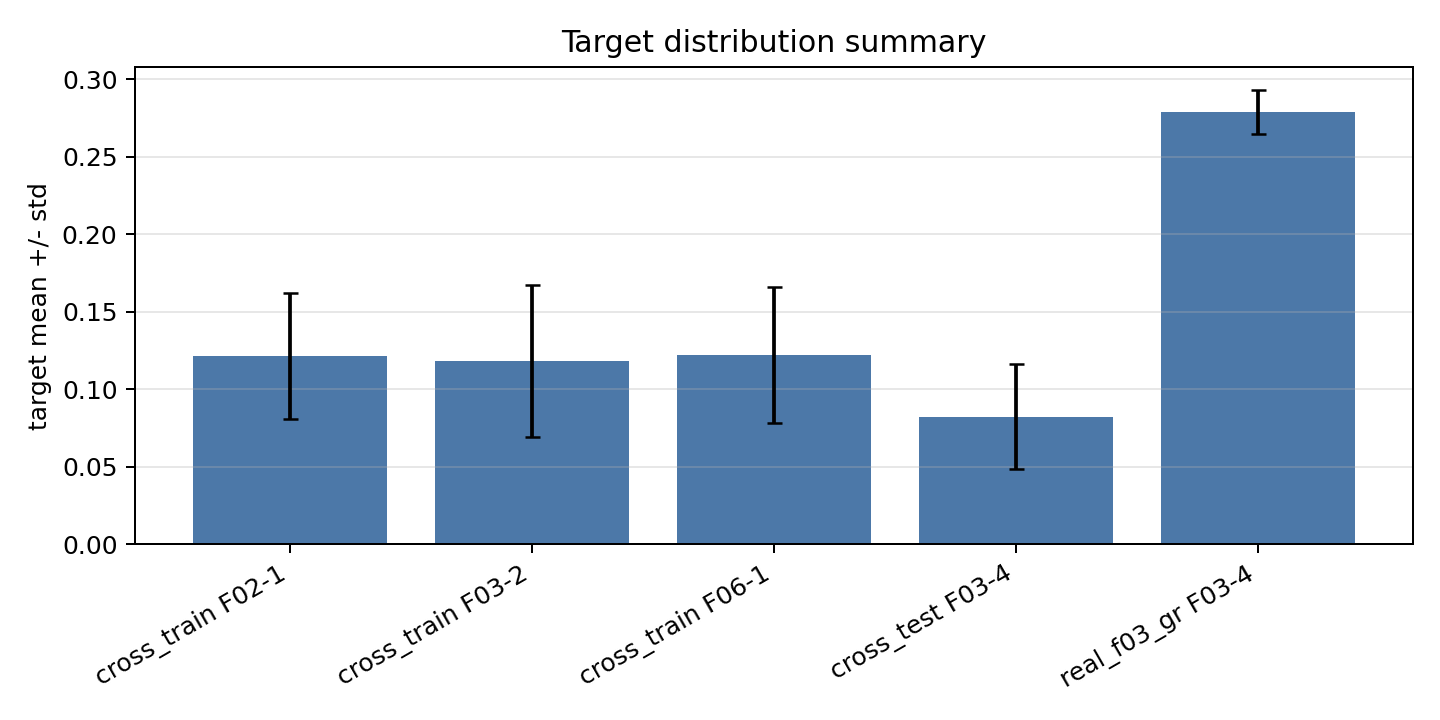
\includegraphics[width=0.86\linewidth]{eda_target_summary.png}
  \caption{Summary of target distributions used in the CLP-CSGM experiments.
  The held-out cross-well Vc target has a lower mean than the training wells,
  while the F03 porosity case has a narrower target range.}
  \label{fig:eda_target_summary}
\end{figure}

Figure~\ref{fig:eda_crosswell_distribution} shows the full Vc distributions for
the cross-well experiment. The held-out F03-4 distribution is shifted toward
lower Vc values relative to the training wells. This shift is important for the
article narrative: the method is not only interpolating within one well, but
using sparse target-well measurements to adapt a learned latent prior under a
visible distribution mismatch.

\begin{figure}[htbp]
  \centering
  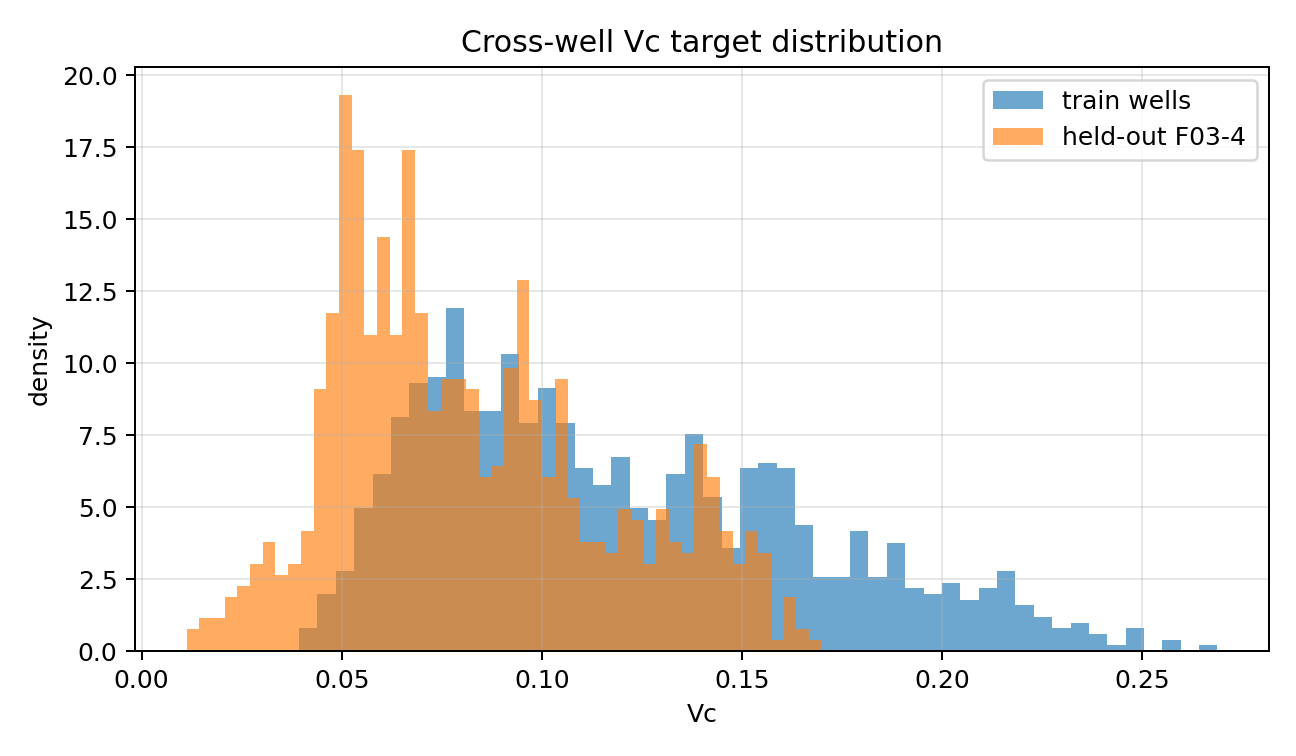
\includegraphics[width=0.78\linewidth]{eda_crosswell_vc_distribution.png}
  \caption{Cross-well Vc target distributions for training wells and held-out
  F03-4. The held-out test distribution is shifted toward lower Vc, motivating a
  measurement-consistent method rather than a purely supervised predictor.}
  \label{fig:eda_crosswell_distribution}
\end{figure}

Table~\ref{tab:eda_correlations} reports simple Pearson correlations between
input channels and targets. Gamma ray is strongly correlated with Vc in both
cross-well train and test splits, whereas the real F03 porosity experiment uses
gamma ray only despite a weak linear correlation with porosity. This GR-only
choice is deliberate: it weakens the dense-input predictor and tests whether
sparse target-well measurements can improve a log-conditioned generative prior.

\begin{table}[htbp]
  \centering
  \caption{Channel-target Pearson correlations. These values are descriptive
  only and are not used as model inputs.}
  \label{tab:eda_correlations}
  \small
  \begin{tabular}{lllr}
\toprule
dataset & channel & target & pearson\_r \\
\midrule
cross\_train & sonic & vc & -0.1642 \\
cross\_train & rhob & vc & 0.0807 \\
cross\_train & gr & vc & 0.9733 \\
cross\_train & ai & vc & 0.1672 \\
cross\_train & vp & vc & 0.1819 \\
cross\_test & sonic & vc & -0.1606 \\
cross\_test & rhob & vc & -0.0061 \\
cross\_test & gr & vc & 0.9772 \\
cross\_test & ai & vc & 0.1330 \\
cross\_test & vp & vc & 0.1077 \\
real\_f03 & ac & porosity & 0.9996 \\
real\_f03 & gr & porosity & -0.1759 \\
\bottomrule
\end{tabular}

\end{table}

Figure~\ref{fig:eda_correlations} visualizes the same channel-target
correlations. In the cross-well Vc task, GR is the dominant linear correlate in
both train and held-out wells, which explains why direct log-based baselines are
not trivial competitors. In the F03 porosity task, however, GR is weakly and
negatively correlated with porosity, whereas AC is almost perfectly correlated.
Using GR only therefore creates a deliberately harder dense-input setting where
the sparse measurements and the latent prior have a clear role.

\begin{figure}[htbp]
  \centering
  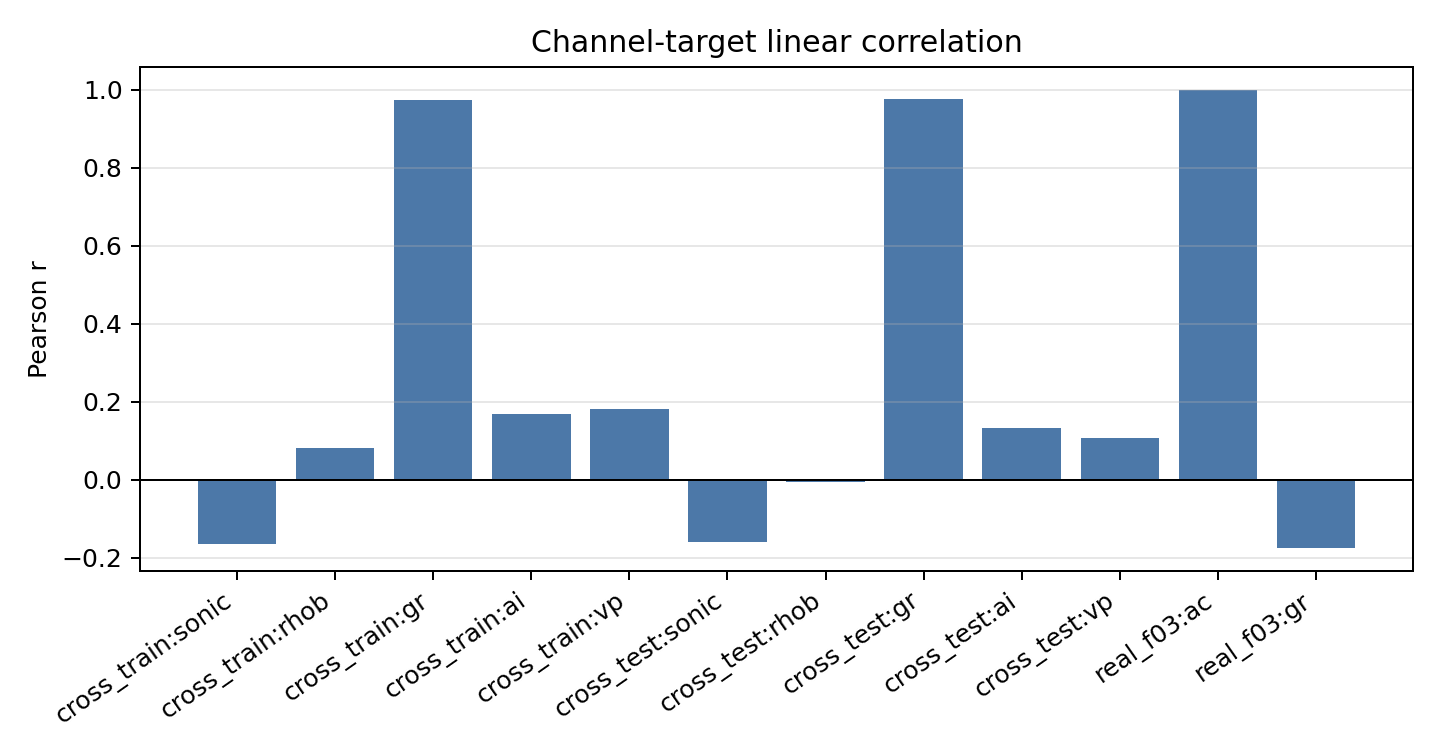
\includegraphics[width=0.88\linewidth]{eda_channel_target_correlations.png}
  \caption{Channel-target Pearson correlations for the cross-well Vc and F03
  porosity data. GR is highly informative for Vc but weak for F03 porosity,
  motivating the GR-only porosity benchmark as a difficult target-well test.}
  \label{fig:eda_correlations}
\end{figure}

Figure~\ref{fig:eda_f03_profile} complements the correlation table by showing
the real F03-4 GR and porosity profiles along depth. The GR-only experiment is
therefore a deliberately weakened dense-input setting: porosity varies smoothly
over the interval, while GR alone is not a near-deterministic porosity proxy.
This makes the sparse porosity observations central to the reconstruction task.

\begin{figure}[htbp]
  \centering
  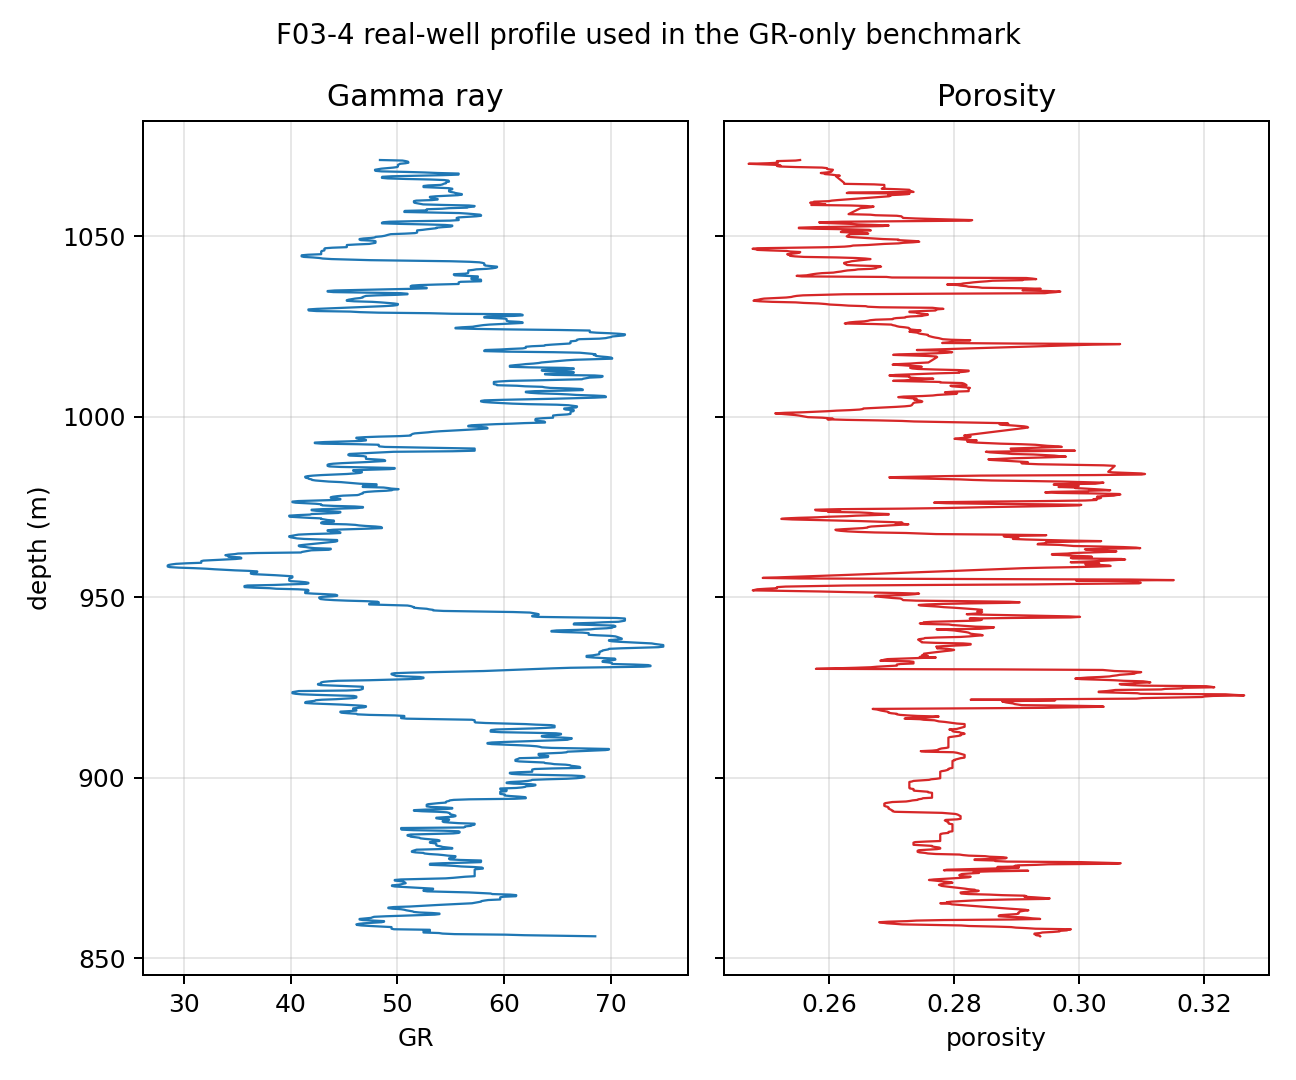
\includegraphics[width=0.82\linewidth]{eda_f03_gr_porosity_depth.png}
  \caption{Real F03-4 depth profiles used in the GR-only porosity benchmark.
  Gamma ray is the only dense input, while porosity is the target profile to be
  reconstructed from sparse observations and the conditional latent prior.}
  \label{fig:eda_f03_profile}
\end{figure}

The EDA therefore supports the experimental design. Cross-well Vc evaluates
low-data transfer under sparse target measurements, while the F03 GR-only case
tests whether CLP-CSGM can recover useful porosity structure when the dense
input alone is intentionally limited.

\section{Experimental setup}
\label{sec:experiments}

\subsection{Cross-well Vc low-data benchmark}

The cross-well benchmark predicts Vc windows of length \(N=64\). Training and
validation windows are built from F02-1, F03-2, and F06-1; F03-4 is held out for
testing. The dense input \(u\) concatenates sonic, density, gamma ray, acoustic
impedance, and \(V_p\) windows. Sparse observations \(b\) are generated by a
coordinate subsampling matrix \(M\) with measurement ratios
\(\rho\in\{0.05,0.10,0.20\}\). The low-data regime is controlled by the sliding
window step: step values \(\{8,16,32\}\) yield approximately
\(\{104,52,27\}\) training windows.

For each step and measurement ratio, results are averaged over seeds
\(\{7,23,41\}\). The CLP-CSGM decoder is trained on standardized training
targets, the ridge prior maps log windows to encoded latents, and \(\lambda\)
is selected by validation RMSE.

\subsection{Real-well F03 GR-only porosity benchmark}

The real-well experiment uses F03-4 AC, GR, and porosity data, but the dense
input is intentionally restricted to GR only. Windows have length \(N=64\) and
are split contiguously by depth: 823 training windows, 274 validation windows,
and 275 test windows. Sparse porosity measurements are simulated by coordinate
subsampling with \(\rho\in\{0.20,0.30,0.40,0.50,0.60\}\). This experiment should
be interpreted as a stress test of sparse-measurement assimilation under weak
dense context, not as a claim that GR-only is the preferred operational
petrophysical configuration.

\subsection{Implementation details}

All target windows are standardized using the training-set mean and standard
deviation before autoencoder training and latent optimization; predictions are
mapped back to the original target scale before metric computation. The
CLP-CSGM generator is a multilayer-perceptron autoencoder with one hidden layer
of width 128 in both encoder and decoder, a latent dimension \(k=16\), ReLU
activations, and a linear output layer. The autoencoder is trained for 200
epochs with Adam, learning rate \(10^{-3}\), weight decay \(10^{-5}\), and batch
size 64.

After autoencoder training, the encoder maps each standardized training target
window to a latent code. The paper-facing prior \(h(u)\) is a Ridge regressor
with \(\alpha=1.0\), fitted from standardized log windows to standardized latent
codes. For the prior-class sensitivity experiment, the MLP prior uses two hidden
layers of width 128, \(L_2\) penalty \(10^{-4}\), learning rate \(10^{-3}\), a
maximum of 500 iterations, and early stopping.

At validation and test time, latent refinement is optimized with Adam for 400
iterations, learning rate \(0.05\), and three restarts. The first restart is
initialized at \(z_0=h(u)\); the remaining restarts add small Gaussian
perturbations. The regularization parameter is selected on the validation split
from
\[
  \lambda\in\{10^{-4},3\cdot10^{-4},10^{-3},3\cdot10^{-3},
  10^{-2},3\cdot10^{-2},10^{-1}\}.
\]
For the measurement-only ablation, \(\lambda=0\) and the latent search is
initialized from zero rather than from \(h(u)\). For the prior-only ablation, no
latent optimization is performed and the prediction is \(G(h(u))\).

\subsection{Baselines and metrics}

The main baselines are:
\begin{itemize}
  \item ML only: supervised MLP using dense logs only.
  \item MLP \([u,b]\): direct MLP using concatenated logs and sparse
  measurements.
  \item PCA \([u,b]\): PCA target representation with an MLP from \([u,b]\) to
  PCA scores.
  \item AE \([u,b]\): autoencoder target representation with an MLP from
  \([u,b]\) to latent codes.
\end{itemize}
The proposed method is reported as CLP-CSGM Ridge. We focus on RMSE, MAE, and
relative \(\ell_2\) error. The previous LFISTA/SIR-CS line is not included in
the main comparison because it is a different proposed method with a fixed-basis
sparse residual prior rather than a conditional generative prior.

\section{Results}
\label{sec:results}

\subsection{Cross-well low-data results}

Table~\ref{tab:crosswell_clp_vs_ae} compares CLP-CSGM Ridge against the
strongest direct baseline, AE \([u,b]\), for every low-data and sparse
measurement cell. CLP-CSGM Ridge wins in all nine cells. The relative RMSE gap
is modest at step 8 and \(\rho=0.05\), but becomes large as the low-data regime
becomes more severe, reaching improvements above 38\% for step 32 at
\(\rho=0.10\) and \(\rho=0.20\).

\begin{table}[htbp]
  \centering
  \caption{Cross-well Vc comparison between CLP-CSGM Ridge and AE \([u,b]\).
  Negative gap means CLP-CSGM has lower RMSE.}
  \label{tab:crosswell_clp_vs_ae}
  \small
  \begin{tabular}{rrrrrr}
\toprule
step & n\_train\_approx & rho & clp\_csgm\_rmse & ae\_ub\_rmse & gap\_vs\_ae\_pct \\
\midrule
8 & 104 & 0.05000 & 0.01541 & 0.01709 & -9.84267 \\
8 & 104 & 0.10000 & 0.01432 & 0.01635 & -12.40651 \\
8 & 104 & 0.20000 & 0.01167 & 0.01633 & -28.52507 \\
16 & 52 & 0.05000 & 0.01493 & 0.01891 & -21.01886 \\
16 & 52 & 0.10000 & 0.01391 & 0.01803 & -22.81414 \\
16 & 52 & 0.20000 & 0.01247 & 0.01808 & -31.00344 \\
32 & 27 & 0.05000 & 0.01562 & 0.02132 & -26.71650 \\
32 & 27 & 0.10000 & 0.01484 & 0.02501 & -40.67353 \\
32 & 27 & 0.20000 & 0.01259 & 0.02035 & -38.15454 \\
\bottomrule
\end{tabular}

\end{table}

\begin{figure}[htbp]
  \centering
  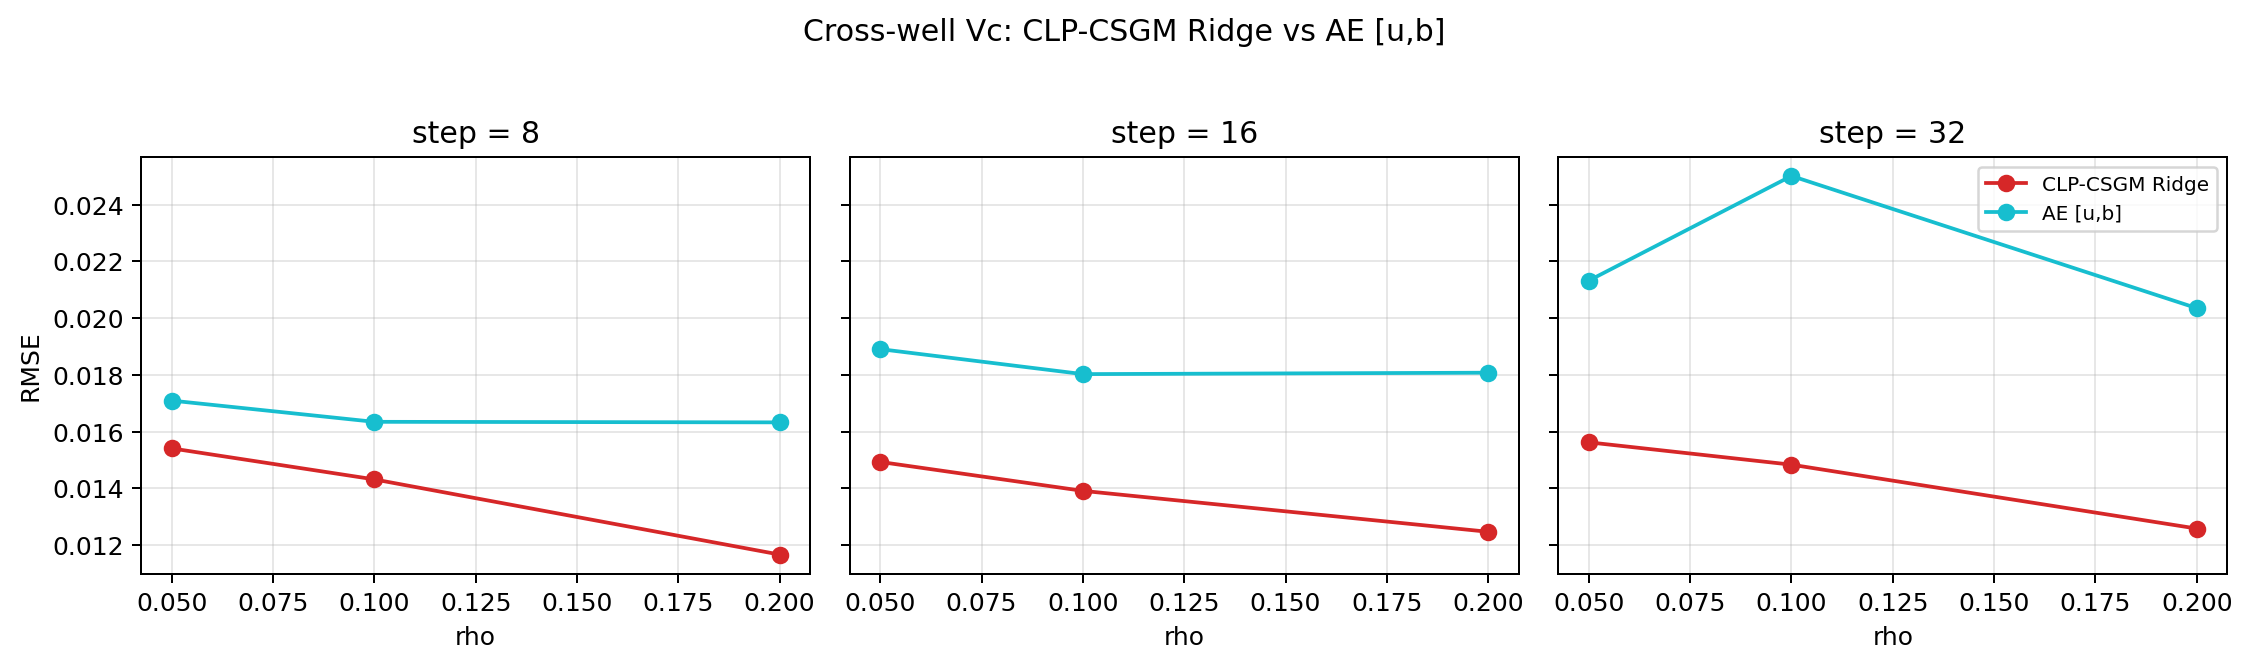
\includegraphics[width=\linewidth]{results_crosswell_clp_vs_ae.png}
  \caption{Cross-well Vc RMSE for CLP-CSGM Ridge and AE \([u,b]\) across the
  low-data grid. Each panel fixes the sliding-window step and varies the sparse
  measurement ratio.}
  \label{fig:crosswell_clp_vs_ae}
\end{figure}

Figure~\ref{fig:crosswell_all_methods} places this pairwise comparison in the
full benchmark context. The direct MLP and PCA baselines become unstable in the
low-data cells, while ML only remains more stable but less accurate. The main
competitor is AE \([u,b]\), and CLP-CSGM Ridge consistently stays below it
across the measurement ratios. This supports the claim that the gain is not an
artifact of comparing against weak baselines; it is visible against the
strongest direct representation-learning baseline.

\begin{figure}[htbp]
  \centering
  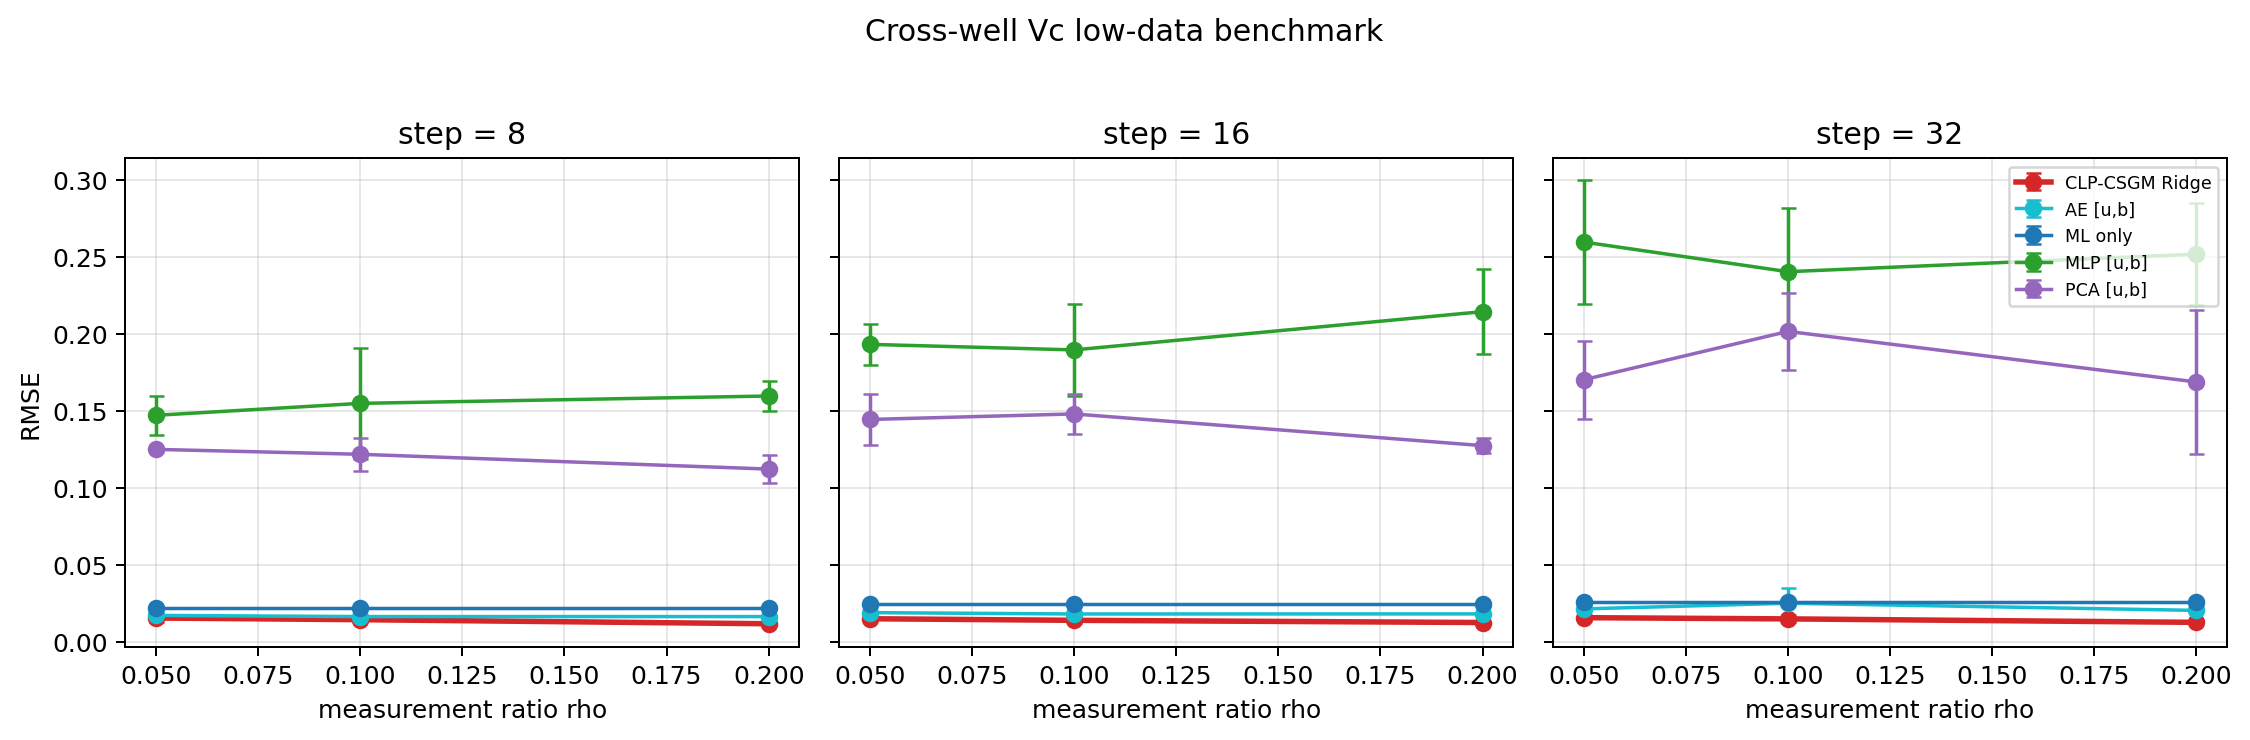
\includegraphics[width=\linewidth]{results_crosswell_rmse_vs_rho.png}
  \caption{Cross-well Vc RMSE for all main benchmarks. CLP-CSGM Ridge remains
  the best method across the low-data grid, while direct MLP and PCA baselines
  degrade sharply when training windows are scarce.}
  \label{fig:crosswell_all_methods}
\end{figure}

The overall ranking in Table~\ref{tab:crosswell_rank} shows the same pattern.
Across the nine step--\(\rho\) cells, CLP-CSGM Ridge obtains mean RMSE
0.01397, compared with 0.01905 for AE \([u,b]\). This corresponds to a relative
gap of about 26.65\% against the strongest direct baseline.

\begin{table}[htbp]
  \centering
  \caption{Overall cross-well Vc ranking across all low-data cells.}
  \label{tab:crosswell_rank}
  \small
  \begin{tabular}{lrrr}
\toprule
method & mean\_rmse & mean\_relative\_l2 & cells \\
\midrule
CLP-CSGM Ridge & 0.01397 & 0.18131 & 9 \\
AE [u,b] & 0.01905 & 0.25464 & 9 \\
ML only & 0.02403 & 0.32932 & 9 \\
PCA [u,b] & 0.14654 & 2.08220 & 9 \\
MLP [u,b] & 0.20112 & 2.79301 & 9 \\
\bottomrule
\end{tabular}

\end{table}

\subsection{Real-well F03 GR-only results}

Table~\ref{tab:f03_results} reports the F03-4 GR-only porosity benchmark.
CLP-CSGM Ridge has the best mean RMSE across measurement ratios, 0.01360 versus
0.01398 for AE \([u,b]\). The gain is concentrated in the sparse-measurement
regime: CLP-CSGM Ridge is clearly better at \(\rho=0.20\) and \(\rho=0.30\).
At higher measurement ratios, AE \([u,b]\) becomes slightly better.

\begin{table}[htbp]
  \centering
  \caption{Real-well F03-4 GR-only porosity benchmark by measurement ratio.}
  \label{tab:f03_results}
  \small
  \begin{tabular}{rlrrr}
\toprule
rho & method & rmse & mae & relative\_l2 \\
\midrule
0.20000 & CLP-CSGM Ridge & 0.01575 & 0.01365 & 0.05909 \\
0.20000 & AE [u,b] & 0.01797 & 0.01560 & 0.06737 \\
0.20000 & PCA [u,b] & 0.02079 & 0.01712 & 0.07791 \\
0.20000 & ML only & 0.02546 & 0.02219 & 0.09550 \\
0.20000 & MLP [u,b] & 0.03189 & 0.02731 & 0.11949 \\
0.30000 & CLP-CSGM Ridge & 0.01449 & 0.01245 & 0.05437 \\
0.30000 & AE [u,b] & 0.01536 & 0.01330 & 0.05760 \\
0.30000 & PCA [u,b] & 0.02241 & 0.01834 & 0.08398 \\
0.30000 & ML only & 0.02546 & 0.02219 & 0.09550 \\
0.30000 & MLP [u,b] & 0.03184 & 0.02716 & 0.11924 \\
0.40000 & AE [u,b] & 0.01296 & 0.01107 & 0.04856 \\
0.40000 & CLP-CSGM Ridge & 0.01342 & 0.01141 & 0.05034 \\
0.40000 & PCA [u,b] & 0.02206 & 0.01790 & 0.08263 \\
0.40000 & ML only & 0.02546 & 0.02219 & 0.09550 \\
0.40000 & MLP [u,b] & 0.03728 & 0.03245 & 0.13966 \\
0.50000 & AE [u,b] & 0.01234 & 0.01065 & 0.04625 \\
0.50000 & CLP-CSGM Ridge & 0.01246 & 0.01061 & 0.04673 \\
0.50000 & PCA [u,b] & 0.02358 & 0.01909 & 0.08834 \\
0.50000 & ML only & 0.02546 & 0.02219 & 0.09550 \\
0.50000 & MLP [u,b] & 0.04466 & 0.03965 & 0.16717 \\
0.60000 & AE [u,b] & 0.01126 & 0.00955 & 0.04218 \\
0.60000 & CLP-CSGM Ridge & 0.01186 & 0.01006 & 0.04447 \\
0.60000 & PCA [u,b] & 0.02417 & 0.01960 & 0.09056 \\
0.60000 & ML only & 0.02546 & 0.02219 & 0.09550 \\
0.60000 & MLP [u,b] & 0.04423 & 0.03873 & 0.16568 \\
\bottomrule
\end{tabular}

\end{table}

\begin{figure}[htbp]
  \centering
  
\includegraphics[width=0.92\linewidth]{01_rmse_vs_measurement_ratio.png}
  \caption{Real-well F03-4 GR-only porosity RMSE by measurement ratio. CLP-CSGM
  Ridge is strongest at the sparsest ratios, while AE \([u,b]\) becomes
  competitive as more target measurements are available.}
  \label{fig:f03_gr_only_rmse}
\end{figure}

Figure~\ref{fig:f03_all_methods} shows the same F03 result with all main
benchmarks. CLP-CSGM Ridge dominates the sparse regime, while AE \([u,b]\)
overtakes it at higher measurement ratios. The crossover is informative rather
than problematic: it marks the regime where enough target-well samples are
available for a direct feature-based model to be competitive.

\begin{figure}[htbp]
  \centering
  
\includegraphics[width=0.92\linewidth]{05_rmse_grouped_bars_by_ratio.png}
  \caption{Real-well F03-4 GR-only RMSE for all main benchmarks. CLP-CSGM Ridge
  has its strongest advantage at low measurement ratios, whereas AE \([u,b]\)
  becomes slightly better when more sparse target measurements are available.}
  \label{fig:f03_all_methods}
\end{figure}

The MAE and relative-\(\ell_2\) curves in
Figs.~\ref{fig:f03_mae}--\ref{fig:f03_rell2} confirm that the RMSE behavior is
not metric-specific. CLP-CSGM Ridge stays close to or below AE \([u,b]\) across
the sparse-to-moderate ratios, while the direct MLP baseline deteriorates as
more sparse-measurement features are added. This suggests that naively
concatenating \(b\) to \(u\) can inject high-variance features, whereas the
proposed method uses \(b\) only through the physical measurement residual.

\begin{figure}[htbp]
  \centering
  
\includegraphics[width=0.92\linewidth]{02_mae_vs_measurement_ratio.png}
  \caption{Real-well F03-4 GR-only MAE by measurement ratio. The ranking is
  consistent with RMSE: CLP-CSGM Ridge is strongest in the sparse regime and
  remains competitive as the measurement ratio increases.}
  \label{fig:f03_mae}
\end{figure}

\begin{figure}[htbp]
  \centering
  
\includegraphics[width=0.92\linewidth]{03_relative_l2_vs_measurement_ratio.png}
  \caption{Relative \(\ell_2\) error on the real-well F03-4 GR-only benchmark.
  The relative-error view preserves the same conclusion as RMSE and MAE,
  indicating that the gain is not caused by scale effects alone.}
  \label{fig:f03_rell2}
\end{figure}

Figures~\ref{fig:f03_gain_rmse}--\ref{fig:f03_gain_mae} express the same
results as gain over the ML-only baseline. Positive values indicate improvement
over using GR alone. CLP-CSGM Ridge and AE \([u,b]\) are the only methods with
large positive gains across all ratios, but CLP-CSGM Ridge has the stronger gain
when measurements are sparse. The direct MLP \([u,b]\) curve is negative,
reinforcing that sparse measurements should be incorporated through a
measurement model rather than only as raw input features.

\begin{figure}[htbp]
  \centering
  
\includegraphics[width=0.92\linewidth]{06_gain_rmse_over_ml_only.png}
  \caption{RMSE gain over the ML-only baseline on F03-4. CLP-CSGM Ridge gives
  the largest gain at low measurement ratios and remains consistently positive
  across the full range.}
  \label{fig:f03_gain_rmse}
\end{figure}

\begin{figure}[htbp]
  \centering
  
\includegraphics[width=0.92\linewidth]{07_gain_mae_over_ml_only.png}
  \caption{MAE gain over the ML-only baseline on F03-4. The gain pattern mirrors
  the RMSE gain, supporting the robustness of the comparison across metrics.}
  \label{fig:f03_gain_mae}
\end{figure}

The qualitative diagnostics in Figs.~\ref{fig:f03_examples}--\ref{fig:f03_depth}
show how these aggregate gains appear in reconstructed profiles. The example
windows show that MLP \([u,b]\) can produce oscillatory outputs, while PCA and
AE are smoother. CLP-CSGM Ridge is also smooth but reacts to sparse constraints
through the latent optimization. The parity plot shows the highest pooled
correlation among the displayed models, and the depth profile indicates that
CLP-CSGM tracks the observed porosity trend without the high-frequency
instability of the direct MLP baseline.

\begin{figure}[htbp]
  \centering
  
\includegraphics[width=\linewidth]{08_example_ground_truth_vs_models.png}
  \caption{Example F03-4 test windows. CLP-CSGM Ridge produces smooth
  reconstructions that follow the ground-truth trend, while direct MLP
  \([u,b]\) is visibly more oscillatory.}
  \label{fig:f03_examples}
\end{figure}

\begin{figure}[htbp]
  \centering
  
\includegraphics[width=0.82\linewidth]{09_parity_ground_truth_vs_prediction.png}
  \caption{Pooled parity plots for F03-4 test windows. CLP-CSGM Ridge has the
  highest displayed correlation, indicating better ordering of high and low
  porosity values across the test block.}
  \label{fig:f03_parity}
\end{figure}

\begin{figure}[htbp]
  \centering
  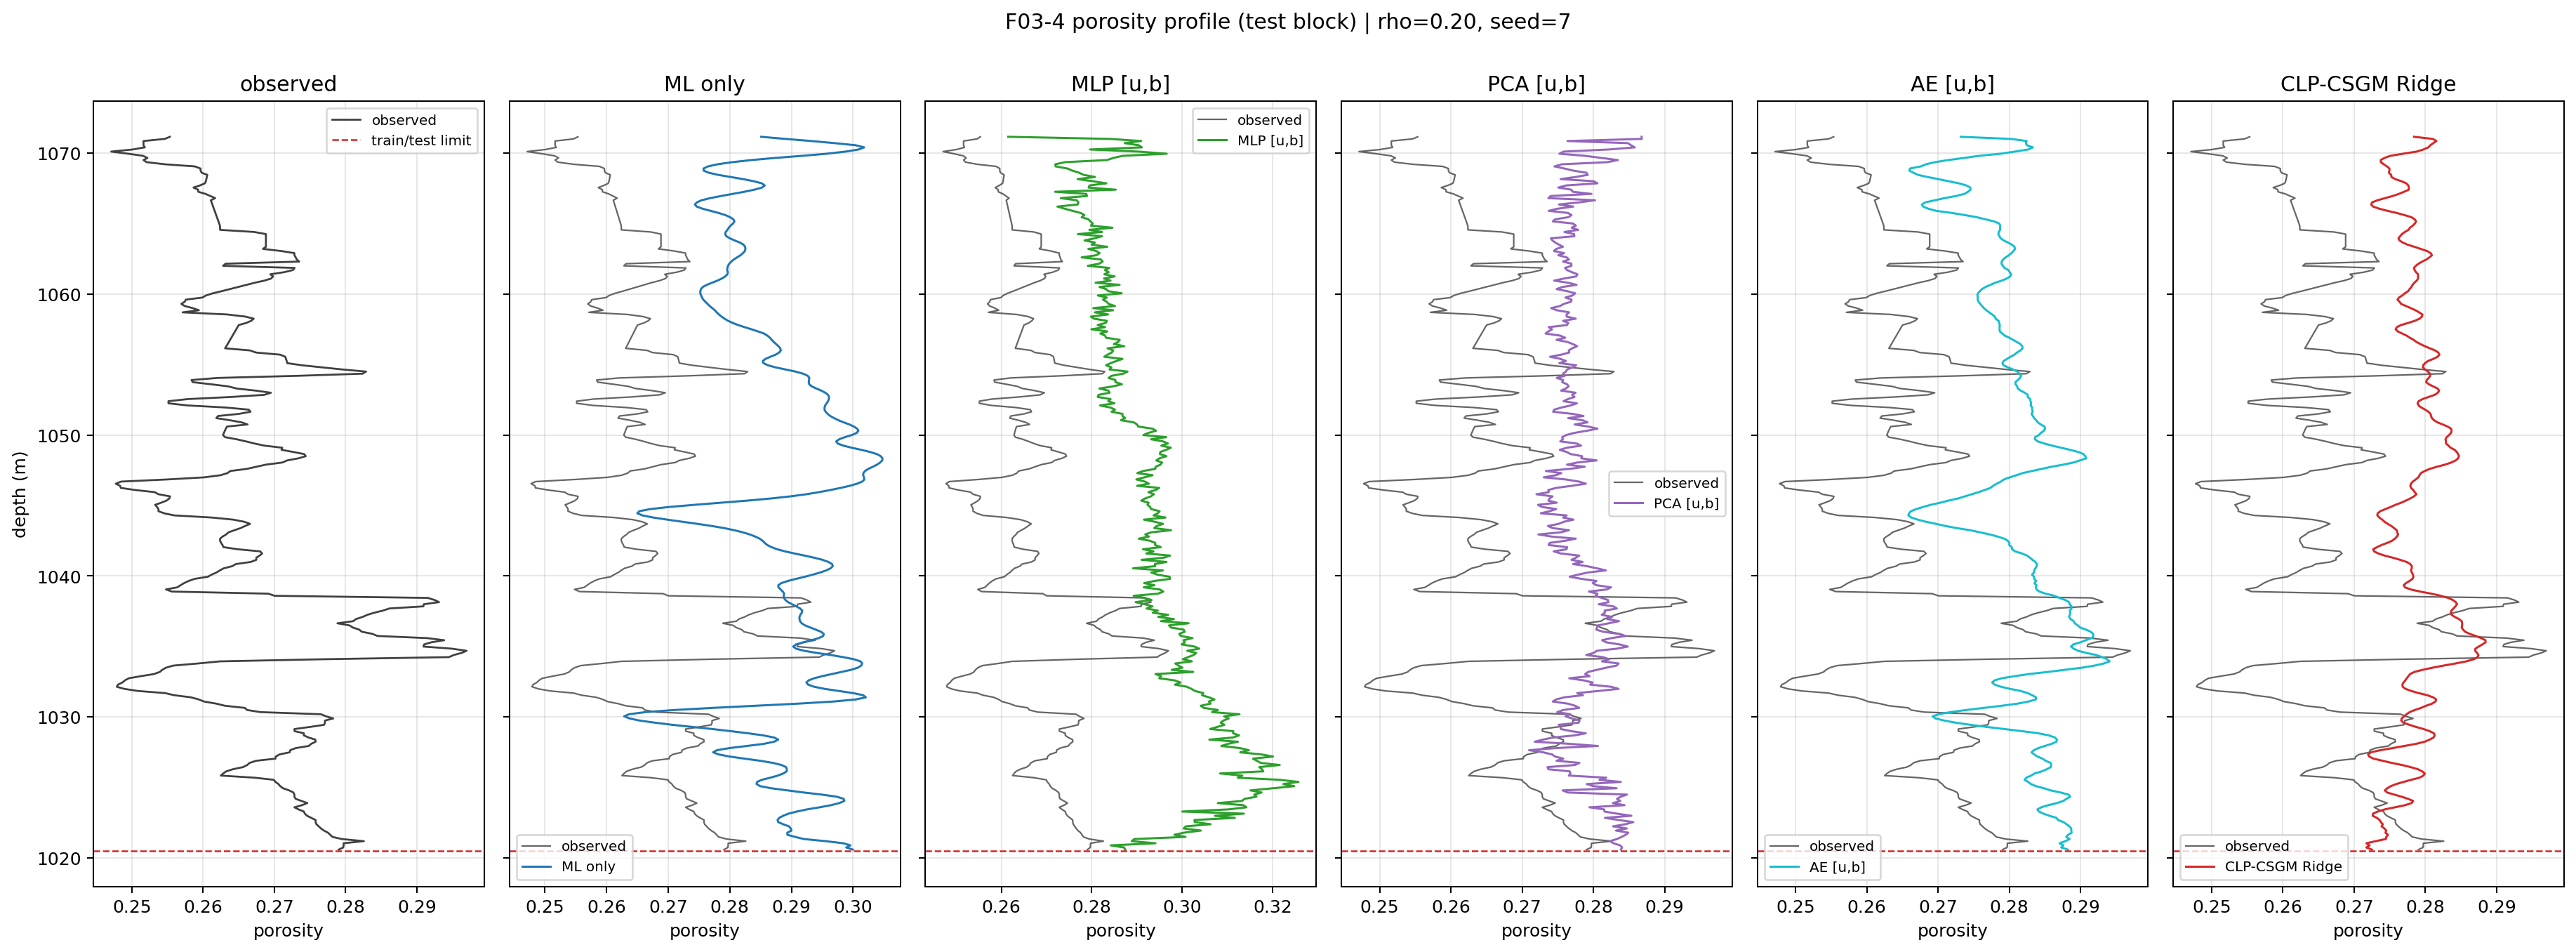
\includegraphics[width=\linewidth]{10_depth_profile_porosity.png}
  \caption{Depth-profile reconstruction for the F03-4 test block at
  \(\rho=0.20\). CLP-CSGM Ridge follows the observed porosity trend while
  avoiding the unstable oscillations of direct MLP \([u,b]\).}
  \label{fig:f03_depth}
\end{figure}

This behavior is consistent with the design of CLP-CSGM. When measurements are
very sparse, the log-conditioned latent prior prevents the inverse problem from
fitting arbitrary sparse observations, while the measurement-consistency term
corrects the weak GR-only prior. When measurements become denser, a direct AE
baseline can use the \([u,b]\) feature vector effectively and the extra latent
optimization may offer less advantage.

\section{Discussion}
\label{sec:discussion}

The results support the central hypothesis: sparse target-well measurements are
more useful when they are enforced through a measurement-consistency term over a
learned latent manifold than when they are used only as additional supervised
features. In the cross-well Vc benchmark, the training set is small and the
held-out well has a shifted target distribution. Direct baselines must learn a
complete \([u,b]\to y\) map from few windows. CLP-CSGM Ridge decomposes the task
into two simpler components: learn a plausible target manifold from training
windows, then select a nearby latent code that is consistent with sparse
measurements in the target well.

The ridge prior is important in this decomposition. It provides a stable
log-conditioned center \(z_0(u)\) in regimes where a more flexible predictor
could overfit. The sparse measurements then act as a local correction rather
than as the only source of information. This explains why the method performs
especially well in low-data and low-\(\rho\) settings.

The real-well F03 experiment gives a more nuanced result. CLP-CSGM Ridge is the
best method on average and is strongest when \(\rho\) is small. However, AE
\([u,b]\) slightly outperforms it at larger \(\rho\). This loss is not
inconsistent with the method objective. CLP-CSGM is designed for sparse
assimilation under a generative prior; when many target samples are available,
a direct model can exploit them without paying the cost or bias of staying near
the learned latent manifold.

Several limitations remain. First, the autoencoder is intentionally small, so
representation error may limit reconstruction of unusual geological patterns.
Second, the theoretical guarantees of CSGM rely on assumptions such as suitable
measurement operators and generator ranges; our coordinate subsampling and
field data do not directly satisfy a proven guarantee. Third, latent
optimization is nonconvex and more expensive than direct regression. Finally,
the experiments use a limited number of wells, so broader geological validation
is needed before claiming field-wide generality.

These limitations also clarify the contribution. CLP-CSGM Ridge is not a
replacement for all direct petrophysical regressors. It is a targeted method
for regimes where dense logs provide a useful but incomplete prior and sparse
core measurements should be honored as physical evidence in the target well.

\section{Conclusion}
\label{sec:conclusion}

We introduced CLP-CSGM Ridge, a conditional generative compressed sensing method
for petrophysical property estimation from dense logs and sparse core
measurements. The method learns a target-property decoder, predicts a
log-conditioned latent prior with ridge regression, and refines the latent code
at test time by enforcing sparse measurement consistency.

In cross-well low-data Vc prediction, CLP-CSGM Ridge outperformed the strongest
direct \([u,b]\) autoencoder baseline in all tested training-size and
measurement-ratio cells. In the real-well F03 GR-only porosity case, it
achieved the best average RMSE, with its clearest advantage in the sparsest
measurement regimes. These results indicate that conditional latent generative
priors are a promising alternative to fixed-basis sparse residual recovery for
petrophysical sparse-measurement assimilation.

Future work should evaluate the method on additional fields, compare richer
conditional priors, investigate uncertainty quantification in latent space, and
study measurement designs beyond coordinate subsampling.


\bibliographystyle{plainnat}
\bibliography{references}

\end{document}
